\chapter{Introduction} \label{sec:introduction}

The fundamental goal of the physical sciences is to understand the laws that govern physical phenomena.
This process inherently involves a continuous interplay between theoretical models and physical observations, forming a feedback loop that continuously refines both. By comparing observational data with model predictions, model validity can be tested, areas of improvements can be identified, and their faithfulness to reality can be improved. Conversely, theoretical models can guide observational strategies by predicting phenomena that have yet to be observed, hence focusing the attention to specific phenomena or conditions that may yield new insights.

A key ingredient of this scientific process is \emph{statistics}. Statistics is a rigorous mathematical language that enables formal statements about what events are possible under physical laws, thus bridging the gap between physics models and observational data.
Guided by this formalization, given some parameters that describe a physical system, implied \emph{predictions} or consequences of a physical model can be computed, allowing for the systematic exploration of the model's implications. Predictions are almost never exact and are intrinsically stochastic, \eg\ due to the randomness of the physical processes, the measurement processes, or incomplete information.
%This approach is known as forward modeling and the above-mentioned physical parameters are called the model parameters.
In order to refine theoretical models, it is essential to perform the inverse process: starting with the effects to discover the causes, inferring from a set of observations the causal factors that produced them. This task, known as solving an \emph{inverse problem}, involves mapping back observational data to infer the underlying model parameters that are not directly observable \cite{Groetsch:1993, Aster:2005}.


\section{Astrophysical data analysis challenges}\label{sec:astro}

In astrophysics and cosmology, this iterative cycle between prediction and inference is particularly challenging due to the complex nature of the systems under study. 
Additionally, we are at the dawn of a data-driven era in astrophysics and cosmology. The coming decade will see transformative science conducted by recent and upcoming observatories, based both on the ground (\eg\ Rubin-LSST \cite{LSSTDarkEnergyScience:2012kar}, ELT \cite{Simon:2019aa}), and space-based missions (\eg\ JWST \citep{Gardner:2006ky}, Euclid \cite{Refregier:2010ss}). Astrophysical data will increase not only in quantity, but also in complexity and detail, promising unprecedented high-precision measurements of the growth of structure and geometry of the universe. This will open new windows to dark matter, dark energy, neutrino physics, inflationary cosmology, and gravity tests. 
Given the unprecedented size and detail of these data, connecting theoretical models with this wealth of high-precision observations presents significant challenges. First, information must be optimally extracted from the data to avoid discarding valuable insights. Second, uncertainties must be correctly treated and thoroughly propagated to ensure accurate scientific statements. Hence, the need for principled statistical analyses has never been more critical. Maximizing information extraction from future experiments, and making robust scientific statements with well quantified uncertainties, are crucial for our ability to uncover new physics. Fully exploiting this data for scientific purposes will require increasingly detailed and complex physical models, which bring along higher computational costs, as well as a larger number of uncertain parameters, including those characterizing signal and background systematics. Developing corresponding theoretical and computational tools to address these challenges for the statistical analysis of astrophysical data is the focus of this thesis.

Figure~\ref{fig:intro-data}

\begin{figure}
    \centering
	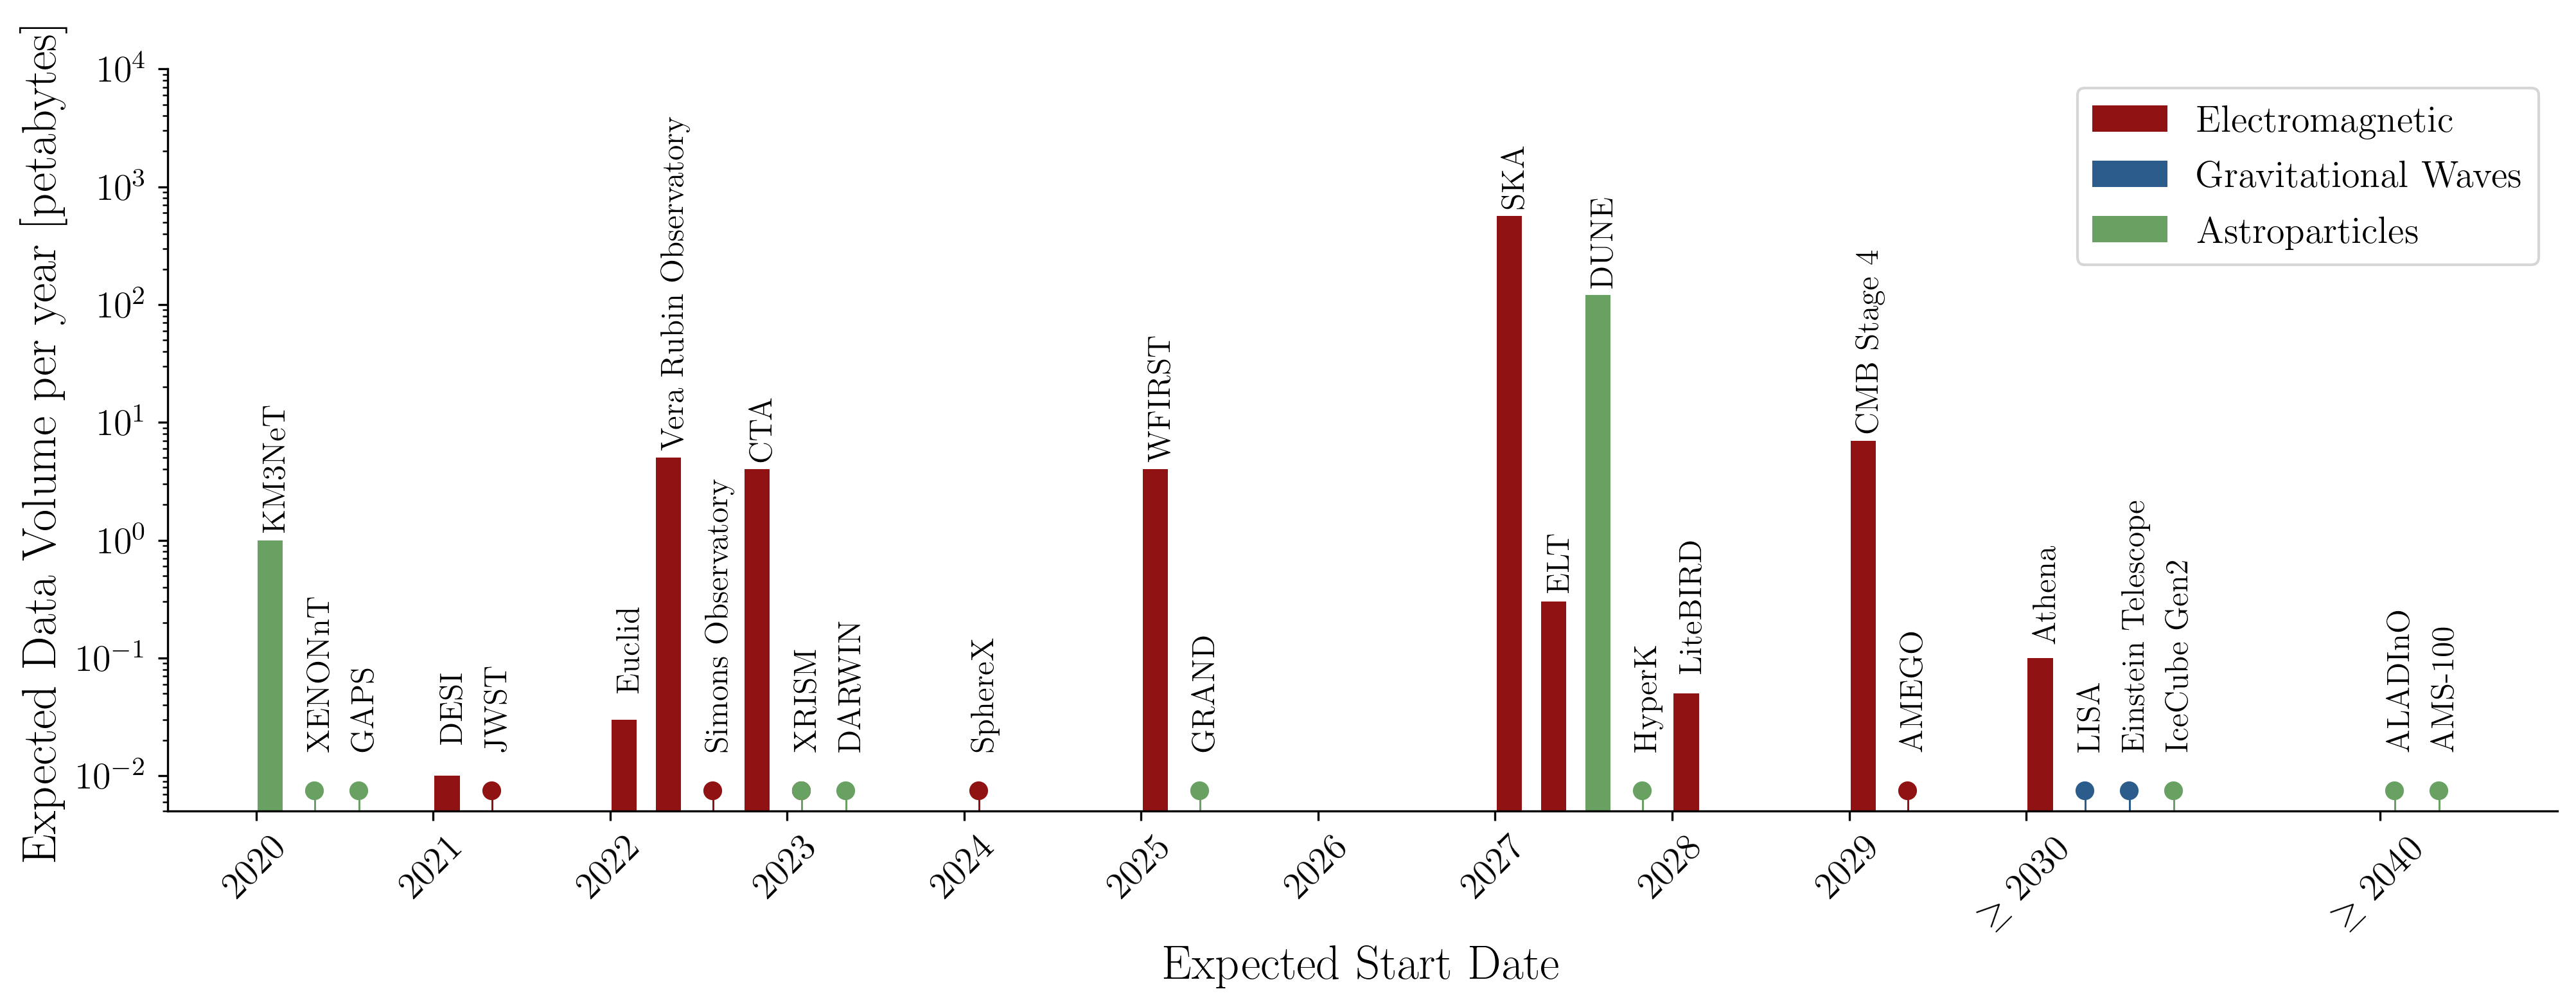
\includegraphics[width=\linewidth]{INTRO-data.png}
    \caption{.}
    \label{fig:intro-data}
\end{figure}












\section{The emergence of the simulation-based inference paradigm}
In recent years, remarkable progress in computing technologies and programming languages have made it possible to express these increasingly detailed and complex physical models through computer \emph{simulators}. Physics simulators serve as powerful predictive devices, mapping model parameters into realized data by reproducing numerically the underlying natural phenomenon of interest. However, while simulators excel at predicting system behaviors, they are poorly suited for statistical inference and for solving inverse problems. 
Broadly speaking, to evaluate the likelihood of a data realization implicitly defined through a computer simulator one must solve an inverse problem that involves integrating all possible code paths, for all possible simulator configurations, that could have potentially led to the observed data realization. Clearly, as the fidelity and detail of modern computer simulations increase, computing this quantity becomes exceedingly difficult, if not entirely intractable or computationally infeasible. 
%Broadly speaking, identifying data-consistent model configurations requires numerical evaluation of the so-called likelihood function—which captures the relative consistency of any given model configuration with observations.
%Unfortunately, conventional statistical inference often poses prohibitively strict restrictions on which models can be used. 
%This creates a dilemma: When we design models with statistical considerations in mind, we have a close feedback loop between data and theory. However, this poses tight constraints on what models can be used. This strategy often only yields limited insights about underlying causal mechanisms. In contrast, when we design interpretable mechanistic models predestined for this purpose, for example, relying on high-fidelity computer simulations, we lose the ability to perform (likelihood-based) statistical inference. Constraining these models by observed data often poses an extremely difficult challenge.

Fortunately, we live in an age of extreme technological innovation and unprecedented computational capabilities. In particular, recent advances in  deep learning and differentiable programming have led to the emergence and proliferation of a \emph{simulation-based inference paradigm} that can effectively tackle the above challenges. By leveraging the power of neural networks, these new methods can approximate the complex relationships within simulators, allowing for efficient solutions to inverse problems that were previously beyond reach.

Motivated by this paradigm shift in statistical analysis, this thesis intends to illustrate possible paths towards further refinement of the scientific loop for astrophysical data in a simulation-based setting. Furthermore, it aims to highlight the potential of neural simulation-based inference in improving the quality of insight we can gain from simulations, maximizing information extraction from data, and providing robust uncertainty quantification for scientific statements.


%Example
%To give the reader some additional intuition as to why the likelihood is intractable, let us briefly consider a metaphor that has been popularized by Kyle Cranmer and Gilles Louppe amongst others. It starts from the premises that the popular Galton board, as depicted in
%Figure 1.3, could be viewed as a scientific simulator. The possible set of simulator outputs correspond to the various bins of the Galton board into which the beads can end up, whereas the simulator’s configu- ration or free parameters relate to the position or bias of the various pegs. To simplify the discussion, let us make the assumption that there are n + 1 bins for n rows of pegs. Contrary to most simulators, the likelihood of a bead ending up in a particular bin does have a tractable likelihood whenever we consider an idealized Galton board. Under this assumed model, the probability of a bead ending up in bin k when counting from the left is defined as
%nkpk(1 − p)n−k, (1.1)
%where p is the probability of a bead bouncing to the right. Recall that the evaluation of the likelihood depends on the integration of all possible code paths that could have produced the observed data. If we view the bead traveling through the Galton board as an execution trace of a computer program with stochastic function calls, then the number of possible paths the computer code can take to produce a bead in bin k is fully described by the binomial coefficient (nk). However, evaluating this likelihood analytically would not be possible if we were to change the position or bias of various pegs. In that case we would not be able to analytically describe the likelihood in the same way, but we would still be able to sample from the simulation model by simply dropping beads into the Galton board!
%
%While the Galton board metaphor demonstrates that even for conceptual problems the computation of the likelihood quickly becomes impractical, the metaphor does not imply that statistical inference in these settings is impossible. In fact, one can still rely on approximate inference as long as it is likelihood-free. This is easier said than done as virtually all statistical inference relies on the likelihood in some way. However, the idea is that surrogates can be constructed that do not rely on the direct evaluation of the likelihood but rather produce estimates of key quantities necessary for statistical inference, be it numerically or otherwise. For instance, one such intractable quantity that is central to this dissertation is the Bayesian posterior
%p(\theta | x) ≜ p(\theta) p(x | \theta), (1.2) p(x)
%where the marginal model
%p(x)≜Z d\theta p(\theta)p(x|\theta), (1.3)
%for a given prior p(\theta) quantifying the initial belief about the free parameters \theta.
%

\section{To likelihood-base or to simulation-base?}\label{sec:lbi-sbi}

%\section{Bayesian analysis}\label{sec:lbi-bayes}

In scientific analyses, inferring the probability distribution of model parameters $\param$ for a given observation $\data_0$ is a ubiquitous task. 
%It is therefore important to begin this chapter by clearly clarifying the adopted definition of probability. Throughout this thesis, we will adopt a Bayesian view of probability. In the Bayesian paradigm, probability is a measure of plausibility and simply quantifies an observer belief about how well a quantity of interest can be measured.
In a Bayesian inference paradigm, the posterior distribution for model parameters $\param$ follows from Bayes' theorem
\begin{equation} \label{eq:sbi-Bayes}
    p(\param\mid\data)=\cfrac{p(\data\mid\param)}{p(\data)} \, p(\param) \, ,
\end{equation}
where $p(\data\mid\param)$ is the likelihood of the data $\data$ for given parameters $\param$, $p(\param)$ is the prior probability distribution over the parameters, and $p(\data)$ is the evidence of the data.  
As evident from Equation \eqref{eq:sbi-Bayes}, the Bayesian framework needs both a formalization of the modeling assumptions, encoded by the likelihood, and a prior knowledge associated with each learnable parameter of the model, encoded by the prior. %It acknowledges that learning a model is a subjective task. Occam’s razor says we should always favour the simplest of potential explanations. The Bayesian approach may naturally handle this principle by attributing higher plausibility to simpler model instantiations.

\begin{figure}
	\centering
	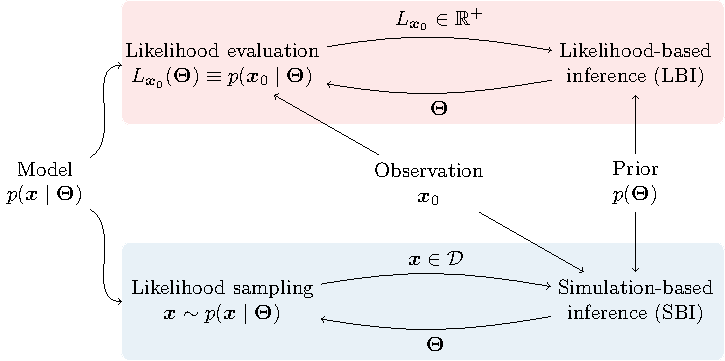
\includegraphics[width=\linewidth]{TikZ/lbi_vs_sbi.pdf}
	\caption{\emph{Likelihood-based} inference algorithms rely on the evaluated likelihood  $L_{\data_0}(\param) $, which is a single scalar that quantifies closeness to the observation $\data_0$. \emph{Simulation-based} inference algorithms learn a function that can be evaluated on many different observations $\data_0$, determining their optimal distance measures case by case. Diagram credits: Christoph Weniger.}
	\label{fig:SBIvsLBI}
\end{figure}

\begin{figure}
    \centering
    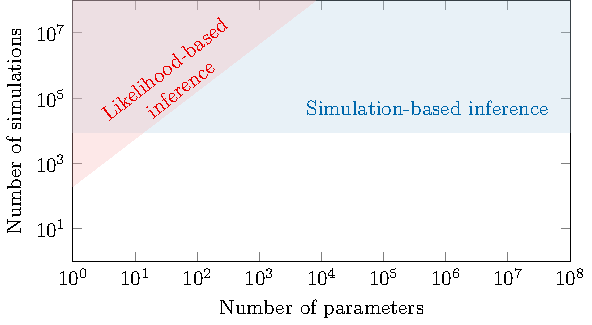
\includegraphics[width=0.9\linewidth]{TikZ/curse_of_dim.pdf}
	\caption{Simplified comparison of likelihood-based and simulation-based algorithms in the space of number of required simulations versus number of model parameters. In general, the simulation requirements of likelihood-based techniques grows significantly with the number of model parameters (curse of dimensionality). Instead, simulation-based inference techniques can, in principle, directly focus on estimating marginal posteriors for parameters of interest, independently of the total number of parameters. This reduces the need for parameter reduction techniques and enables the comparison of complex simulation results with complex data. The figure is adapted from Figure 4 in Ref.~\cite{Boddy:2022knd}.}
    \label{fig:sbi-lbi-cost}
\end{figure}
 
Given this Bayesian setup, statistical inference is performed within the context of a probabilistic model $p(\data\mid\param)$, that can be in principle accessed by two different routes. On one hand, \gls*{lbi} algorithms rely on likelihood \underline{evaluations}, single scalars that quantify closeness to the observation $\data_0$. The main \gls*{lbi} tools to solve inverse problems for modern astrophysical and cosmological data analysis have been sampling-based inference methods like \gls*{mcmc} \citep{Metropolis:1953am, Hastings:1970aa} and nested sampling \citep{Skilling:2006gxv, Feroz:2008xx, Handley:2015fda} techniques. However, these methods often rely on approximate likelihoods, and the time needed to reach convergence scales poorly with the dimensionality of the explored parameter space. More modern methods are taking up this latter challenge, including gradient-based algorithms such as Hamiltonian Monte-Carlo~\citep{Duane:1987de}, or slice-sampling techniques~\citep{Neal:aa, Handley:2015fda}.

\subsection{Likelihood-based methods}

\subsection{Simulation-based methods}

On the other hand, \gls*{sbi} algorithms do not explicitly calculate the likelihood function, but instead rely on \underline{samples} from a stochastic simulator that  \emph{implicitly maps} model parameters $\param$ to data $\data$. This mapping is equivalent to sampling from the model distribution $\data \sim p(\data\mid\param)$, which is effectively an implicit representation of the likelihood. As a result, in this setting one just need a computational code that generates random samples from $p(\data\mid\param)$, that can be later used by a \gls*{sbi} algorithm. For the purpose of this thesis, a \emph{simulator/forward model} is a computer program that takes as input a vector of parameters $\param \in \mathbb{R}^D$, samples a series of internal states or latent variables, and finally produces a data vector  $\data$  as output (usually our observable). Programs that involve random samplings and are interpreted as statistical models are known as probabilistic programs, and simulators are an example \cite{Cranmer:2019eaq}. In principle, using simulators allows for the simultaneous inclusion of all relevant processes that can affect the data, regardless of whether a full probabilistic description is tractable or not, as long as they can be efficiently programmed. In this context, \emph{intractability} means one of two things: a closed-form expression of the likelihood distribution is not available, or even if available it is computationally too expensive, \eg\, in the worst case, it scales exponentially with the number of parameters \cite{Leclercq:2018who, Mootoovaloo:2020ott}.

\subsection{Comparison}
The main differences between \gls*{sbi} and \gls*{lbi} methods are summarized in Figure~\ref{fig:SBIvsLBI}. In both cases, we start with a data model, $p(\data\mid\param$), which describes the probability of data $\data$ given parameters $\param$. In the \gls*{lbi} case, the strategy is a detailed analysis of the likelihood function $L_{\data_0}(\param)$, given an observation $\data_0$. To this end, simplifying, the \gls*{lbi} algorithm will suggest points $\param$ where the likelihood will be evaluated, and try to focus on regions with high density. On the other hand, \gls*{sbi} techniques do \emph{not} require a tractable (see above) likelihood-density $p(\data_0\mid\param)$ at a specific observation $\data_0$. Instead, they rely on synthetic data samples from the likelihood function $\data \sim p(\data\mid\param)$, for a range of model parameters $\param$ that are in the simplest case drawn from the parameter priors, $\param \sim p(\param)$, or in more complex cases from generative models \cite[\eg][]{Karchev:2022aa}. % Essentially, simulation-based techniques are calibrated based on samples from the \emph{generative model} or \emph{joined distribution} $\data, \param \sim p(\data\mid\param)p(\param) \equiv p(\data, \param)$.  

%While \gls*{lbi} produces results with maximal precision and usually the failure mode is over-confidence, the standard failure mode for \gls*{sbi} algorithms is under-confidence (provided correlations between $\data$ and $\param$ are fully identified).

%Classical likelihood-based inference algorithms are problem-agnostic: their performance does not directly depend on the properties, dimensionality or shape of the data $\data \sim p(\data\mid\param)$ for different model parameters $\param$; instead it \textit{only} depends on the shape of the likelihood function as a function of $\param$ for a specific piece of observation $\data_0$, $p(\data_0\mid\param)$.  This is in stark difference to simulation-based, or likelihood-free, algorithms, where the performance of a given algorithm depends critically on how (simulated and real) data $\data$ is processed, interpreted and used.  On first sight, this suggests that simulation-based algorithms are in general more difficult to use, since there are more choices to make.  However, if properly used, simulation-based techniques offer a range of advantages over likelihood-based methods, which we group here into three dimensions, which are also illustrated in 

While in principle the two frameworks converge to the same answer, when applied several practical differences emerge. We will highlight now two of the most striking disparities, but others will surface in the remaining sections of this chapter when the discussion becomes more technical.

\noindent \textbf{Recyclable inference.} As highlighted in Figure~\ref{fig:SBIvsLBI}, the analyzed observation $\data_0$ enters the statistical framework of \gls*{lbi} and \gls*{sbi} at different stages. In particular, \gls*{lbi} algorithms perform inference for a fixed observation $\data_0$, and must rerun from scratch for any another observation. It is thus computationally costly to perform new analysis and statistical test on the obtained results. On the other hand, we will see that \gls*{sbi} algorithms effectively learn an estimate of the probability density function that can be used to perform ``online" inference on any new data (as long as they stem from the same prior support). In this case, there is no need to rerun the whole pipeline for different observations, but just to re-evaluate the learned function on new data.\footnote{This property is not fully preserved in case of sequential \gls*{sbi} algorithms, as they prioritize achieving other types of benefits (this will be illustrated in Chapter~\ref{cha:sbi}).} Furthermore, statistical consistency tests can be performed rather quickly and efficiently. This aspect will be explored in Section~\ref{subsec:tmnre-test}.

\noindent \textbf{Breaking the curse of dimensionality.} When using likelihood-based techniques, in order to solve \emph{one} inference problem, like obtaining samples for marginal posterior of interest, one has to solve \emph{all} of them (joint posterior estimate). The computational overhead of generating joint samples as an intermediate step of marginal inference can be enormous, and can quickly turn an apparently easy inference task, like the measurement of a single physical parameter, into a big challenge. These cases are not uncommon, and require problem specific care, like analytically performing parts of the marginal integrals. \todo{justify with lensing}

On the other hand, one key aspect of \gls*{sbi} algorithms in general is their ability to \emph{directly estimate marginal posteriors} for parameters of interest, instead of having to first estimate the joint posterior over all parameter space, and then marginalize out nuisance parameters. The possibility to directly estimate marginal probabilities effectively means that we can use \gls*{sbi} algorithms to break down large problems into smaller ones, while coherently accounting for the uncertainties coming from the rest of the parameter space (as further detailed in Section~\ref{subsec:tmnre-m}). This specificity makes SBI techniques extremely scalable and simulation efficient with respect to likelihood-based ones as a function of model parameters, as exemplified in Figure~\ref{fig:sbi-lbi-cost}. 







\section{Outline}
This thesis aims to contribute to the ongoing effort to transition towards simulation-based inference techniques in astrophysics and cosmology, emphasizing some of the tremendous opportunities that this transition brings. To this end, this thesis first proposes a general simulation-based ecosystem for astrophysical data analysis (Chapter~\ref{cha:sbi}). Then, it illustrate its capabilities through three exemplary applications to astrophysics: 
\begin{itemize}[leftmargin=1cm]
	\item the analysis of strong gravitational lenses as a dark matter probe in Chapters~\ref{cha:lensing} and \ref{cha:anre}, 
	\item the reconstruction of cosmological initial conditions from late-time density fields in Chapter~\ref{cha:cosmo}, 
	\item and the analysis of point-sources in sky-maps in Chapter~\ref{cha:detection}. 
\end{itemize}
Overall, it aims to highlight the potential for fast, flexible, and testable simulation-based algorithms to facilitate scientific discovery in astrophysics and cosmology, at the dawn of their data-driven era, and forward.




